\documentclass{article}

\usepackage{color}
\usepackage{graphicx}
\usepackage{amsmath}
\usepackage{geometry}
\usepackage{setspace}
\usepackage{indentfirst}
\usepackage{listings}
\usepackage{xcolor}
\lstset{
    columns=fixed,       
    numbers=left,                                       
    frame=none,                                          
    backgroundcolor=\color[RGB]{245,245,244},            
    keywordstyle=\color[RGB]{40,40,255},                 
    numberstyle=\footnotesize\color{darkgray},           
    commentstyle=\it\color[RGB]{0,96,96},                
    stringstyle=\rmfamily\slshape\color[RGB]{128,0,0},   
    showstringspaces=false,                              
    language=c++,                                        
}
\geometry{left=2cm,right=2cm,top=2cm,bottom=2cm}
\begin{document}
\begin{spacing}{2.0}
\vspace*{0.25cm}

\hrulefill

\thispagestyle{empty}

\begin{center}
\begin{large}
\sc{UM--SJTU Joint Institute \vspace{0.3em} \\ Data Structures and Algorithms \\(VE281)}
\end{large}

\hrulefill

\vspace*{5cm}
\begin{Large}
\sc{{Homework 1}}
\end{Large}

\vspace{2em}

\end{center}


\vfill

\begin{table}[h!]
\flushleft
\begin{tabular}{lll}
Name: Ji Xingyou \hspace*{2em}&
ID: 515370910197\hspace*{2em}
\\

Date: 26 September 2017

\end{tabular}
\end{table}

\hfill

\newpage
\tableofcontents
\newpage
\section{Theoretical Data}
\indent As is discussed in the class, we can get the following table summarizing the time complexity for each sorting algorithms.

\begin{table}[!hbp]
\centering
\begin{tabular}{ccccc}
&Worst case complexity&Average case complexity&In place&Stable\\
\hline
\hline
Bubble sort&$O(N^2)$&$O(N^2)$&Yes&Yes\\
\hline
Insertion sort&$O(N^2)$&$O(N^2)$&Yes&Yes\\
\hline
Selection sort&$O(N^2)$&$O(N^2)$&Yes&No\\
\hline
Merge sort&$O(NlogN)$&$O(NlogN)$&No&Yes\\
\hline
Quick sort extra&$O(N^2)$&$O(NlogN)$&No&No\\
\hline
Quick sort in place&$O(N^2)$&$O(NlogN)$&Yes&No\\
\hline
\end{tabular}
\caption{Time complexity of comparison sorting}
\end{table}

In this report, we will first implement all these six sorting algorithms, and then test the run time for each of them to see whether the above table makes sense.

The implementation of the algorithms is attached in the appendix.
\section{Result Analysis}
\indent After finishing implementing the above six sorting algorithms, I wrote another program to test the run time of each algorithm. In this program, I set two clocks, noting the starting and finishing instance. To avoid uncertainty in the data, I wrote a while loop to run the program 10 times so that I could get the average value. There is one thing which requires extra carefulness. That is, we must ensure that every time inside the while loop, all the six sorting should meet the identical array. Otherwise, you will see that insertion sort will have a leading performance no matter how large the size is.

The array size I chose is 1, 10, 100, 1000, 5000, 10000, 50000, 100000.

The run time data for each sorting algorithms is listed in table 2.
\begin{table}[!h]
\centering
\begin{tabular}{c|cccccc}
Array size&Bubble sort&Insertion sort&Selection sort&Merge sort&Quick sort extra&Quick sort in place\\
\hline
\hline
1&1&0&0&0&0&1\\
\hline
10&1&0&0&5&2&2\\
\hline
100&34&11&20&40&20&11\\
\hline
1000&2744&880&1300&384&231&137\\
\hline
5000&72741&18552&27256&1706&1085&698\\
\hline
10000&308764&72484&107564&3951&2284&1404\\
\hline
50000&8705506&1802895&2661684&20023&12562&8597\\
\hline
100000&34518575&7144271&10326454&39702&25401&17999\\
\hline
\end{tabular}
\caption{Run time of comparison sorting}
\end{table}

The run time comparison is shown in figure 1. Notice that in the Matlab code, I used semilogy instead of plot command. The reason is that when using plot command, most data all gathered near the x-axis, which adds to the difficulty in observing.
\begin{figure}[h!]
\begin{center}
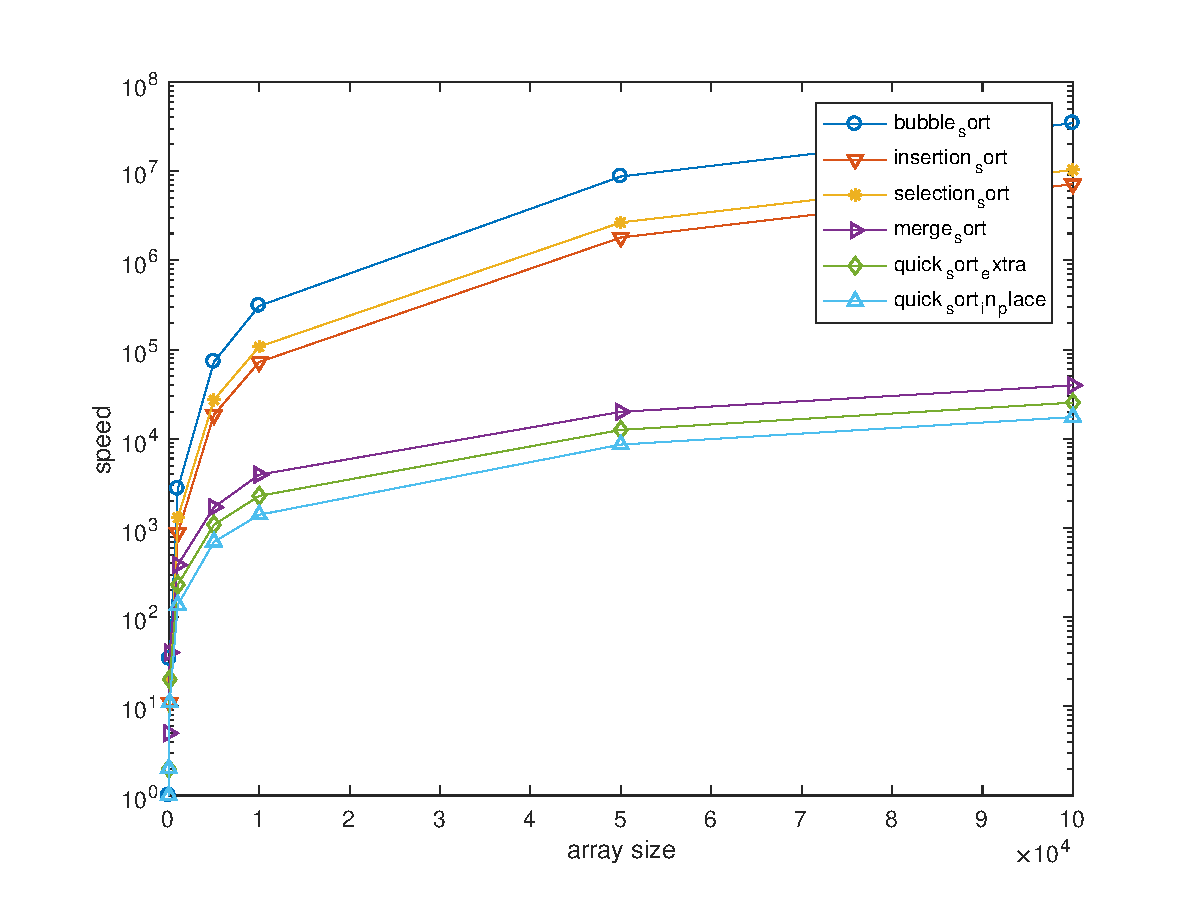
\includegraphics[scale=1]{run_time.eps}
\caption{Run time comparison}
\end{center}
\end{figure}

Combining the table and figure above, we can conclude the following points.
\begin{enumerate}
\item For each sorting algorithm, the run time increases as the size of the array increases.\\
\item When the array size is small (less than 1000), bubble sort, insertion sort and selection sort have a better performance than merge sort, quick sort with extra space and quick sort in place.\\
\item When the array size becomes gradually larger (greater than 10000), merge sort, quick sort with extra space and quick sort in place have a much better performance than bubble sort, insertion sort and selection sort.\\
\item It can be inferred from the data and the figure that when the array size is very large (greater than 100000), bubble sort has the least performance, selection sort the second, insertion sort the third, merge sort the fourth, quick sort with extra space the fifth and quick sort in place the best.\\
\end{enumerate}

From the conclusion listed above, we can see that it fits the time complexity shown in table 1, which means the algorithms make sense.

This inspires me that in future learning, when dealing with sorting, I should make a wise choice on which sorting algorithm to apply. For example, if there is no restriction on stablity and in place, when the array size is small, I should use insertion sort and selection sort. When the array size is large, I should choose merge sort, quick sort with extra space and quick sort in place.
\section{Appendix}
\subsection{Sorting algorithms}
\begin{lstlisting}[language=c++]
//
//  main.cpp
//  project1
//
//  Created by 季星佑 on 2017/9/11.
//  Copyright © 2017年 季星佑. All rights reserved.
//

#include <iostream>
#include <fstream>
#include <sstream>
#include <string>
#include <cstdlib>
#include <climits>
#include <ctime>
#include <cassert>

using namespace std;

void bubble_sort(int *arr,int lines);

void insertion_sort(int *arr,int lines);

void selection_sort(int *arr,int lines);

void merge(int *C,int *A,int len_A,int *B,int len_B,int lines);

void merge_sort(int *arr,int lines);

int quick_sort_partition_extra(int *arr,int left,int right,int lines);

void quick_sort_extra(int *arr,int left,int right,int size);

int quick_sort_partition_in_place(int *arr,int left,int right,int lines,int pivotat);

void quick_sort_in_place(int *arr,int left,int right,int size);
//////////////////////////////
//////////////////////////////
int main(int argc, const char * argv[])
{
    int choice;
    cin>>choice;
    int lines;
    cin>>lines;
    int a[lines];
    for(int i=0;i<lines;++i)
    {
        cin>>a[i];
    }
    int *arr=a;
    switch(choice)
    {
        case 0:
            bubble_sort(arr,lines);
            break;
        case 1:
            insertion_sort(arr,lines);
            break;
        case 2:
            selection_sort(arr,lines);
            break;
        case 3:
            merge_sort(arr,lines);
            break;
        case 4:
            quick_sort_extra(arr,0,lines-1,lines);
            break;
        case 5:
            quick_sort_in_place(arr,0,lines-1,lines);
            break;
        default:
            break;
    }
    for(int k=0;k<lines;++k)
    {
        cout<<arr[k]<<endl;
    }
    return 0;
}
//////////////////////////////
//////////////////////////////
void bubble_sort(int *arr,int lines)
{
    for(int i=lines-1;i>0;--i)
    {
        for(int j=0;j<i;++j)
        {
            if(arr[j]>arr[j+1])
            {
                swap(arr[j],arr[j+1]);
            }
        }
    }
}
//////////////////////////////
//////////////////////////////
void insertion_sort(int *arr,int lines)
{
    for(int i=0;i<=lines-1;++i)
    {
        int temp=arr[i];
        int j=i;
        while(j>=1)
        {
            if(arr[j-1]>temp)
            {
                arr[j]=arr[j-1];
                --j;
            }
            else
            {
                break;
            }
        }
        arr[j]=temp;
    }
}
//////////////////////////////
//////////////////////////////
void selection_sort(int *arr,int lines)
{
    for(int i=0;i<lines-1;++i)
    {
        int index=i;
        for(int j=i+1;j<lines;++j)
        {
            if(arr[j]<arr[index])
            {
                index=j;
            }
        }
        if(index!=i)
        {
            int tmp=arr[index];
            arr[index]=arr[i];
            arr[i]=tmp;
        }
    }
}
//////////////////////////////
//////////////////////////////
void merge(int *C,int *A,int len_A,int *B,int len_B,int lines)
{
    int i=0,j=0,k=0;
    while(i<len_A&&j<len_B)
    {
        if(A[i]<B[j])
        {
            C[k++]=A[i++];
        }
        else
        {
            C[k++]=B[j++];
        }
    }
    while(i<len_A)
    {
        C[k++]=A[i++];
    }
    while(j<len_B)
    {
        C[k++]=B[j++];
    }
}

void merge_sort(int *arr,int lines)
{
    if(lines<=1)
    {
        return;
    }
    int mid=lines/2;
    int *A=new int[mid];
    int *B=new int[lines-mid];
    for(int i=0;i<mid;++i)
    {
        A[i]=arr[i];
    }
    for(int i=mid;i<lines;++i)
    {
        B[i-mid]=arr[i];
    }
    merge_sort(A,mid);
    merge_sort(B,lines-mid);
    merge(arr,A,mid,B,lines-mid,lines);
    delete [] A;
    delete [] B;
}
//////////////////////////////
//////////////////////////////
int quick_sort_partition_extra(int *arr,int left,int right,int lines)
{
    int *temp=new int[lines];
    int l=0;
    int r=lines-1;
    for(int k=1;k<lines;++k)
    {
        if(arr[k]<arr[0])
        {
            temp[l]=arr[k];
            l++;
        }
        else
        {
            temp[r]=arr[k];
            r--;
        }
    }
    temp[l]=arr[0];
    for(int t=0;t<lines;++t)
    {
        arr[t]=temp[t];
    }
    delete [] temp;
    return l;
}

void quick_sort_extra(int *arr,int left,int right,int size)
{
    int pivotat;
    if(left>=right)
    {
        return;
    }
    pivotat=quick_sort_partition_extra(arr,left,right,size);
    quick_sort_extra(arr,left,pivotat-1,pivotat-left);
    quick_sort_extra(arr+pivotat+1,0,right-pivotat-1,right-pivotat);
}
//////////////////////////////
//////////////////////////////
int quick_sort_partition_in_place(int *arr,int left,int right,int lines,int pivotat)
{
    swap(arr[0],arr[pivotat]);
    int i=1;
    int j=lines-1;
    while(true)
    {
        while(i<lines-1&&arr[i]<arr[0])
        {
            ++i;
        }
        while(j>0&&arr[j]>=arr[0])
        {
            --j;
        }
        if(i<j)
        {
            swap(arr[i],arr[j]);
        }
        else
        {
            break;
        }
    }
    swap(arr[0],arr[j]);
    return j;
}

void quick_sort_in_place(int *arr,int left,int right,int size)
{
    if(size==0)
    {
        return;
    }
    int pivotat=rand()%size;
    if(left>=right)
    {
        return;
    }
    pivotat=quick_sort_partition_in_place(arr,left,right,size,pivotat);
    quick_sort_in_place(arr,left,pivotat-1,pivotat-left);
    quick_sort_in_place(arr+pivotat+1,0,right-pivotat-1,right-pivotat);
}

\end{lstlisting}
\subsection{Run-time calculation}
\begin{lstlisting}[language=c++]
//
//  main.cpp
//  runtime_study
//
//  Created by 季星佑 on 2017/9/23.
//  Copyright © 2017年 季星佑. All rights reserved.
//

#include <iostream>
#include <fstream>
#include <sstream>
#include <string>
#include <cstdlib>
#include <climits>
#include <ctime>
#include <cassert>

using namespace std;

void bubble_sort(int arr[],int lines);

void insertion_sort(int arr[],int lines);

void selection_sort(int arr[],int lines);

void merge(int *C,int *A,int len_A,int *B,int len_B,int lines);

void merge_sort(int arr[],int lines);

int quick_sort_partition_extra(int arr[],int left,int right,int lines);

void quick_sort_extra(int arr[],int left,int right,int size);

int quick_sort_partition_in_place(int arr[],int left,int right,int lines,int pivotat);

void quick_sort_in_place(int arr[],int left,int right,int size);
//////////////////////////////
//////////////////////////////
int main(int argc, const char * argv[])
{
    int lines=50000;
    long temp0=0;
    long temp1=0;
    long temp2=0;
    long temp3=0;
    long temp4=0;
    long temp5=0;
    clock_t start,finish;
    cout<<"lines = "<<lines<<endl;
    int arr[lines];
    for(int i=0;i<lines;++i)
    {
        arr[i]=mrand48();
    }
    int brr[lines];
    for(int j=0;j<lines;++j)
    {
        brr[j]=arr[j];
    }
    int k=0;
    while(k<10)
    {
        //////////////////////////////
        start=clock();
        for(int a=0;a<lines;++a)
        {
            arr[a]=brr[a];
        }
        bubble_sort(arr,lines);
        finish=clock();
        long t0=finish-start;
        temp0+=t0;
        //////////////////////////////
        start=clock();
        for(int a=0;a<lines;++a)
        {
            arr[a]=brr[a];
        }
        insertion_sort(arr,lines);
        finish=clock();
        long t1=finish-start;
        temp1+=t1;
        //////////////////////////////
        start=clock();
        for(int a=0;a<lines;++a)
        {
            arr[a]=brr[a];
        }
        selection_sort(arr,lines);
        finish=clock();
        long t2=finish-start;
        temp2+=t2;
        //////////////////////////////
        start=clock();
        for(int a=0;a<lines;++a)
        {
            arr[a]=brr[a];
        }
        merge_sort(arr,lines);
        finish=clock();
        long t3=finish-start;
        temp3+=t3;
        //////////////////////////////
        start=clock();
        for(int a=0;a<lines;++a)
        {
            arr[a]=brr[a];
        }
        quick_sort_extra(arr,0,lines-1,lines);
        finish=clock();
        long t4=finish-start;
        temp4+=t4;
        //////////////////////////////
        start=clock();
        for(int a=0;a<lines;++a)
        {
            arr[a]=brr[a];
        }
        quick_sort_in_place(arr,0,lines-1,lines);
        finish=clock();
        long t5=finish-start;
        temp5+=t5;
        //////////////////////////////
        k++;
    }
    long time0=temp0/10;
    long time1=temp1/10;
    long time2=temp2/10;
    long time3=temp3/10;
    long time4=temp4/10;
    long time5=temp5/10;
    cout<<time0<<endl;
    cout<<time1<<endl;
    cout<<time2<<endl;
    cout<<time3<<endl;
    cout<<time4<<endl;
    cout<<time5<<endl;
    return 0;
}
//////////////////////////////
//////////////////////////////
void bubble_sort(int *arr,int lines)
{
    for(int i=lines-1;i>0;--i)
    {
        for(int j=0;j<i;++j)
        {
            if(arr[j]>arr[j+1])
            {
                swap(arr[j],arr[j+1]);
            }
        }
    }
}
//////////////////////////////
//////////////////////////////
void insertion_sort(int *arr,int lines)
{
    for(int i=0;i<=lines-1;++i)
    {
        int temp=arr[i];
        int j=i;
        while(j>=1)
        {
            if(arr[j-1]>temp)
            {
                arr[j]=arr[j-1];
                --j;
            }
            else
            {
                break;
            }
        }
        arr[j]=temp;
    }
}
//////////////////////////////
//////////////////////////////
void selection_sort(int *arr,int lines)
{
    for(int i=0;i<lines-1;++i)
    {
        int index=i;
        for(int j=i+1;j<lines;++j)
        {
            if(arr[j]<arr[index])
            {
                index=j;
            }
        }
        if(index!=i)
        {
            int tmp=arr[index];
            arr[index]=arr[i];
            arr[i]=tmp;
        }
    }
}
//////////////////////////////
//////////////////////////////
void merge(int *C,int *A,int len_A,int *B,int len_B,int lines)
{
    int i=0,j=0,k=0;
    while(i<len_A&&j<len_B)
    {
        if(A[i]<B[j])
        {
            C[k++]=A[i++];
        }
        else
        {
            C[k++]=B[j++];
        }
    }
    while(i<len_A)
    {
        C[k++]=A[i++];
    }
    while(j<len_B)
    {
        C[k++]=B[j++];
    }
}

void merge_sort(int *arr,int lines)
{
    if(lines<=1)
    {
        return;
    }
    int mid=lines/2;
    int *A=new int[mid];
    int *B=new int[lines-mid];
    for(int i=0;i<mid;++i)
    {
        A[i]=arr[i];
    }
    for(int i=mid;i<lines;++i)
    {
        B[i-mid]=arr[i];
    }
    merge_sort(A,mid);
    merge_sort(B,lines-mid);
    merge(arr,A,mid,B,lines-mid,lines);
    delete [] A;
    delete [] B;
}
//////////////////////////////
//////////////////////////////
int quick_sort_partition_extra(int *arr,int left,int right,int lines)
{
    int *temp=new int[lines];
    int l=0;
    int r=lines-1;
    for(int k=1;k<lines;++k)
    {
        if(arr[k]<arr[0])
        {
            temp[l]=arr[k];
            l++;
        }
        else
        {
            temp[r]=arr[k];
            r--;
        }
    }
    temp[l]=arr[0];
    for(int t=0;t<lines;++t)
    {
        arr[t]=temp[t];
    }
    delete [] temp;
    return l;
}

void quick_sort_extra(int *arr,int left,int right,int size)
{
    int pivotat;
    if(left>=right)
    {
        return;
    }
    pivotat=quick_sort_partition_extra(arr,left,right,size);
    quick_sort_extra(arr,left,pivotat-1,pivotat-left);
    quick_sort_extra(arr+pivotat+1,0,right-pivotat-1,right-pivotat);
}
//////////////////////////////
//////////////////////////////
int quick_sort_partition_in_place(int *arr,int left,int right,int lines,int pivotat)
{
    swap(arr[0],arr[pivotat]);
    int i=1;
    int j=lines-1;
    while(true)
    {
        while(i<lines-1&&arr[i]<arr[0])
        {
            ++i;
        }
        while(j>0&&arr[j]>=arr[0])
        {
            --j;
        }
        if(i<j)
        {
            swap(arr[i],arr[j]);
        }
        else
        {
            break;
        }
    }
    swap(arr[0],arr[j]);
    return j;
}

void quick_sort_in_place(int *arr,int left,int right,int size)
{
    if(size==0)
    {
        return;
    }
    int pivotat=rand()%size;
    if(left>=right)
    {
        return;
    }
    pivotat=quick_sort_partition_in_place(arr,left,right,size,pivotat);
    quick_sort_in_place(arr,left,pivotat-1,pivotat-left);
    quick_sort_in_place(arr+pivotat+1,0,right-pivotat-1,right-pivotat);
}

\end{lstlisting}
\subsection{Visualization}
\begin{lstlisting}[language=Matlab]
clear all;clc;
t0=[1 1 34 2744 72741 308764 8705506 34518575];
t1=[0 0 11 880 18552 72484 1802895 7144271];
t2=[0 0 20 1300 27256 107564 2661684 10326454];
t3=[0 5 40 384 1706 3951 20023 39702];
t4=[0 2 20 231 1085 2284 12562 25401];
t5=[1 2 11 137 698 1404 8597 17499];
size=[1 10 100 1000 5000 10000 50000 100000];
semilogy(size,t0,'o-',size,t1,'v-',size,t2,'*-',size,t3,'>-',size,t4,'d-',size,t5,'^-');
xlabel('array size');
ylabel('speed');
legend('bubble_sort','insertion_sort','selection_sort','merge_sort',
'quick_sort_extra','quick_sort_in_place');
\end{lstlisting}
\end{spacing}
\end{document}